\chapter{The proximity force approximation}
\label{chapter_pfa}

Another method to calculate the free Casimir energy between arbitrary shaped
smooth objects is the proximity force approximation (PFA). The PFA links
arbitrary geometries to the much simpler plane--plane geometry and also
accounts for thermal effects and finite conductivity of the mirrors. For this
reason, the PFA is commonly used for comparisons with experiments. Although the
approximation is believed to become accurate for small separations, no error
estimates exist \cite{2011PhRvD84j5031F}.

In this chapter, we want to compare numerical results obtained using the
scattering approach with predictions of the PFA. We will only consider perfect
reflectors here. We will see that for small separations the PFA becomes a good
approximation. However, even for separations $L/R \sim 0.02$ the error of the
approximation is still in the percent range.

\section{The PFA for the plane--sphere geometry}

\begin{wrapfigure}{r}{0.382\textwidth}
  \begin{center}
      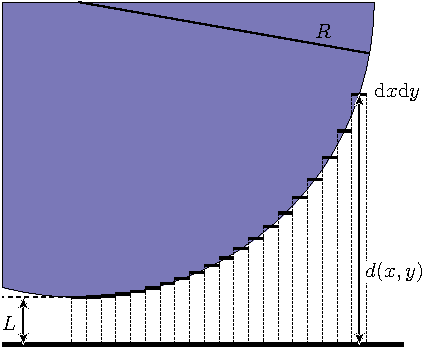
\includegraphics[scale=0.85]{images/pfa.pdf}
  \end{center}
  \caption{PFA for the plane--sphere geometry. The sphere is approximated by infinitesimal plates that are parallel to the plane.}
  \label{fig:pfa_idea}
\end{wrapfigure}
We will follow the derivation from Ref. \cite{CasimirAdvances}. Let us consider two bodies: the
surface of the upper body may be described by $z_1 = z_1(x,y)$ and the surface
of the lower by $z_2 = z_2(x,y)$. Then the separation between both bodies is given by
\begin{equation}
d(x,y) \equiv z_1(x,y)-z_2(x,y).
\end{equation}
For a given point $(x,y)$ we now replace the infinitesimal surface elements
$\mathrm{d}S_1$ of the upper and $\mathrm{d}S_2$ of the lower body by parallel
surface elements $\mathrm{d}x \mathrm{d}y$ around the points $z_1(x,y)$ and
$z_2(x,y)$. Thereby we link the unknown interaction energy to the well-known
energy of the plane--plane geometry. In this way we can calculate the free energy
of this geometry by integration 
\begin{equation}
\mathcal{F}_\text{PFA} = \int_\Sigma \frac{\mathcal{F}_\text{PP}(d(x,y))}{A} \mathrm{d}x \mathrm{d}y,
\end{equation}
where $\Sigma$ is the area of the $xy$-plane where the function $d(x,y)$ is
defined. For the plane--sphere geometry the idea of the PFA is sketched in Fig. \ref{fig:pfa_idea}.

Let us now apply the PFA to the plane--sphere geometry. The separation between
plane and sphere is given by
\begin{equation}
d(x,y) = L+R-\sqrt{R^2-x^2-y^2} = L+R(1-\cos\theta)
\end{equation}
and the integration can be carried out in spherical coordinates
\begin{equation}
\label{eq:pfa_pfa_generic}
\mathcal{F}_\text{PFA} = \int_0^{2\pi} \mathrm{d}\varphi \int_0^{\pi/2} \mathrm{d}\theta \, \frac{\mathcal{F}_\text{PP}\left(L+R(1-\cos\theta)\right)}{A} \, R^2\sin\theta,
\end{equation}
where $R^2 \sin\theta \, \mathrm{d}\theta \mathrm{d}\varphi$ is the surface element in
spherical coordinates. The integrand is independent of $\varphi$ and the
integration over $\theta$ can be simplified by substituting
$t=1+(1-\cos\theta) \, R/L$. Doing so, we obtain for the free energy in the
plane--sphere geometry
\begin{equation}
\label{eq:pfa_pfa_ps}
\mathcal{F}_\text{PFA} = 2\pi RL \int_1^{1+R/L} \mathrm{d}t \, \frac{\mathcal{F}_\text{PP}(Lt)}{A}.
\end{equation}
The evaluation of \eqref{eq:pfa_pfa_ps} is notably simpler than the formulas we
obtained in the scattering formalism. However, the PFA neglects some intrinsic
properties of the plane--sphere geometry:
\begin{itemize}
\item The PFA ignores the finite curvature of the sphere. In particular, the
curvature alters the way waves are scattered. While the curvature causes waves
to be scattered in different directions, wave scattering is resonant in the
PFA. This is the reason why the PFA usually overestimates the value of the free
energy.
\item The PFA uses the free energy of the plane--plane geometry. In this geometry the
polarizations $p=\TE,\TM$ are uncoupled and yield independent contributions to the free
energy. However, in the plane--sphere geometry the polarizations are coupled. This will
become important in the study of the large--distance limit in chapter \ref{chapter_ld}.
\item The Casimir free energy is non-additive. However, the PFA assumes that the
sphere can be divided into small parallel area elements and the contributions of
these area elements with the plane are additive.
\item For perfect reflectors the entropy is always positive in the plane--plane geometry. In the
PFA approximation the free energy is given as an integral over the free energy in the plane--plane geometry and
the entropy obtained is always positive. However, in the plane--sphere geometry the
entropy becomes negative for a wide range of parameters.
\end{itemize}

In the next section we will compare our numerical results obtained using the
scattering approach with the PFA approximation.

\section{Comparison with scattering approach}

\begin{figure}
  \begin{center}
  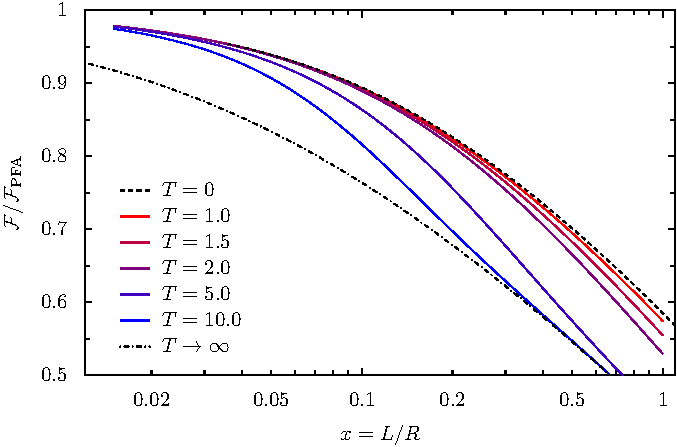
\includegraphics[scale=1]{plots/pfa/pfa.pdf}
  \end{center}

  \caption{Comparison of the PFA approximation with numerical results
  obtained using the scattering formalism versus the aspect ratio $x=L/R$.
  We plot the ratio $\mathcal{F}/\mathcal{F}_\text{PFA}$ for different temperatures, including the
  zero temperature and the high temperature limit. The numerical data for the
  zero temperature limit (for $x>0.035$) are obtained by interpolation (cf. section \ref{section_thermal_low_temp}), the data
  for the high temperature limit are obtained by calculating the $n=0$ Matsubara
  term (cf. section \ref{section_thermal_hi_temp}).}
  \label{fig:pfa_pfa}
\end{figure}

The aspect ratio $L/R$ will play a crucial role in our considerations and for
this reason we define $x\equiv L/R$.
For perfect reflectors we can insert \eqref{eq:scattering_pp_F_perfect}
into \eqref{eq:pfa_pfa_ps} and obtain
\begin{equation}
\mathcal{F}_\text{PFA} = \frac{T}{4\pi \, x} \int_1^{1+x^{-1}} \mathrm{d}t \, \frac{1}{t^2} \sum_n^\prime \left[\text{Li}_3\left(\e^{-2nTtx/(x+1)}\right)+ \frac{2nT t x}{1+x} \text{Li}_2\left(e^{-2nTtx/(x+1)}\right)\right],
\end{equation}
where we use the dimensionless quantities defined in section
\ref{scattering_ps_scaling}. From \eqref{eq:scattering_pp_F_perfect_hiT}
and \eqref{eq:scattering_pp_F_perfect_T0} we find the behaviour for
$T=0$ and high temperatures:
\begin{align}
\label{eq:pfa_T0}
\mathcal{F}_\text{PFA}^{T=0}     &= -\frac{\pi^3}{720} \frac{1+2x}{x^3+x^2} \approx -\frac{\pi^3}{720 \, x^2} \\
\label{eq:pfa_HT}
\mathcal{F}_\text{PFA}^\text{HT} &= -\frac{T \xi(3)}{8\pi} \frac{1}{x^2+x} \approx -\frac{T \xi(3)}{8\pi \, x}
\end{align}
The free energy in the Drude model becomes independent of the particular properties of the metal for
high temperatures and we find
\begin{equation}
\label{eq:pfa_HT_drude}
\mathcal{F}_\text{PFA}^\text{HT,D} = -\frac{T \xi(3)}{16\pi} \frac{1}{x^2+x} \approx -\frac{T \xi(3)}{16\pi \, x}.
\end{equation}
The expressions obtained for the high temperature limit for perfect reflectors
and Drude mirrors differ by a factor of $2$. The reason is the same as in
section \ref{section_scattering_pp_drude}: The Fresnel coefficient for TE
polarization for $\xi\to0$ becomes $r_\TE=0$ in the Drude model, but $r_\TE=-1$
for perfect reflectors.
    
In Fig. \ref{fig:pfa_pfa} we plot the ratio
$\mathcal{F}/\mathcal{F}_\text{PFA}$ in the range $0.015\le L/R \le 1$ for
different temperatures including $T=0$ and the high temperature limit.
The numerical results were obtained using $\lmax =
\text{max}\left(25,\lceil\eta R/L\rceil\right)$ with $\eta=5.8$ and
$\epsilon_p=2\cdot10^{-7}$. For small separations the ratio
$\mathcal{F}/\mathcal{F}_\text{PFA}$ tends to unity. The accuracy of the PFA
becomes better for small separations and for low temperatures. For $L/R=0.015$
the ratio is $0.9788$ for $T=1$, and $0.9747$ for $T=10$. However, the PFA
approximation is a good approximation for small separations and only for small
separations. For separations $L/R\approx0.1$ the ratio $\mathcal{F}/\mathcal{F}_\text{PFA}$ is only about $0.9$
even for very small temperatures. We also want to remind the reader that the
PFA does not cover effects like negative entropies in the plane--sphere geometry.
Moreover, the PFA is in a sense an uncontrolled approximation as no error estimates
exist.

We want to stress one more point: The PFA becomes a good approximation for
small separations. This means that it captures the main physical effects in its
limits of validity. However, entropies obtained using the PFA are always positive.
From that we may conclude that the effect of negative entropies must vanish or
become negligible for small separations. This argument can also be understood
in terms of geometry: Small separations correspond to small curvatures of the
sphere and the plane--sphere geometry becomes similar to the plane--plane
geometry. This is in fact the main idea of the PFA approximation. As no
parameters for which the entropy becomes negative exist in the plane--plane
geometry, we expect negative entropies to disappear for small separations.
We will investigate this question in more detail
in chapter \ref{chapter_negative_entropies}.
